%%=============================================================================
%% AutoKeras
%%=============================================================================

\chapter{AutoKeras}
\label{ch:autokeras}

In dit hoofdstuk wordt het volledige AutoKeras proces uitgelegd. Dit door belangrijke stukken code te nemen en expliciet toe te lichten welke keuzes gemaakt zijn en waarom. Ook \textit{performance metrics} worden hier verzameld en vergeleken. Het model is met verschillende parameter configuraties getraind. Elke variant blijft wel hetzelfde \textit{code skeleton} gebruiken.

De ontwikkeling is volledig in \textit{Jupyter notebooks}\footnote{\url{https://jupyter.org/}} uitgewerkt. Om de code makkelijk lokaal te gebruiken is \textit{Anaconda Navigator\footnote{\url{https://docs.anaconda.com/anaconda/navigator/}}} aangeraden, de meeste \textit{packages} worden standaard mee geïnstalleerd. De code bevindt zich ook in Appendix \ref{ch:app:autokeras} en kan online bekeken worden\footnote{\url{https://github.com/robbedec/bachproef-automl}}.

Volgende \textit{packages} moeten zelf geïnstalleerd worden:

\begin{itemize}
    \item tensorflow-gpu (2.1.0)
    \item autokeras (1.0.2)
    \item graphviz (0.13.2)
\end{itemize}

\section{Voorafgaand werk}
\label{sec:autokeras-before}

\subsection{GPU activatie}
\label{subsec:autokeras-gpu}

Het verloop van de code is ook hoe je een model van nul kan trainen. Er wordt gewerkt met een \textit{CUDA integrated GPU}, om te testen als \textit{tensorflow} wel echt de GPU gebruikt kunnen er enkele commando's uitgevoerd worden. Als in de output een vermelding over de GPU staat mag u er vanuit gaan dat de die actief is.

\bigskip

\begin{python}
from tensorflow.python.client import device_lib

def get_available_devices():
    local_device_protos = device_lib.list_local_devices()
    return [x.name for x in local_device_protos]
print(get_available_devices()) 
\end{python}

Een mogelijkse output kan er als volgt uitzien: ['/device:CPU:0', '/device:GPU:0'].

\subsection{Data transformatie}
\label{subsec:autokeras-tranform}

De dataset bestaat deels uit een gelabeld afbeeldingen. Het bevat ook een verzameling ongelabelde afbeeldingen die tijdens de wedstrijd gebruikt werden als verificatie. In het kader van het onderzoek kan dit weggelaten worden en kunnen we aan de slag gaan met de gelabelde data. Elke afbeelding wordt genormaliseerd naar een standaard resolutie en omgezet naar een \textit{numpy array}\footnote{In de code is 'np' een verwijzing naar \textit{numpy}}. Dit zijn de kleurwaarden van elke pixel die samen een matrix vormen. Ook het label van de afbeelding is opgenomen in de matrix (0 = hond, 1 = kat). Momenteel staat alle data nog gegroepeerd volgens categorie. Voor de volgende stap is het belangrijk dat dit niet het geval is. Daarom wordt de matrix nog eens random gesorteerd.

\bigskip

\begin{python}
def get_label(file):
    class_label = file.split('.')[0]
    if class_label == 'dog': label_vector = 0
    elif class_label == 'cat': label_vector = 1
    return label_vector
    
def get_data():
    data = []
    files = os.listdir(INPUT_PATH)
    
    for image in tqdm(files):
        label_vector = get_label(image)
        img = Image.open(INPUT_PATH + image).convert('L')
        img = img.resize((SIZE,SIZE))
    
        data.append([np.asarray(img),np.array(label_vector)])
        
    shuffle(data)
    return data

\end{python}

\section{Data preprocessing}
\label{sec:preprocessing-autokeras}

Een van de requirements is dat de \textit{preprocessing} voor de gebruiker gedaan wordt. Bij AutoKeras is dit niet het 100\% het geval en moeten er zelf nog enkele zaken uitgevoerd worden. Zo moet de matrix die gemaakt is in sectie \ref{subsec:autokeras-tranform} opgedeeld worden in training en validatie datasets.

In \textit{data science} projecten wordt typisch x\_test en x\_train gebruikt om de \textit{features} van de afbeeldingen op te slaan, de matrix met pixel waarden. y\_test y\_train bevatten dan het bijhorend label. In de tweede stap wordt er dimensiereductie toegepast. De algoritmes houden geen rekening met kleuren dus die mogen we weglaten. De drie kleurendimensies (Rood, Groen, Blauw) worden omgezet naar één dimensie (grijswaarden).

\bigskip

\begin{python}
x_train = np.array([data[0] for data in train], 'float32')
x_test = np.array([data[0] for data in test], 'float32')
y_train = [data[1] for data in train]
y_test = [data[1] for data in test]

x_train = np.array(x_train).reshape(-1,SIZE,SIZE,1)
x_test = np.array(x_test).reshape(-1,SIZE,SIZE,1)

x_train /= 255
x_test /= 255
\end{python}

\section{Model trainen en evalueren}
\label{sec:traineval-autokeras}

Met alle voorbereiding afgewerkt is het tijd om \textit{classifier} in gang te steken. Hierbij moet enkel een naam (voor het uiteindelijke model) en het maximum aantal pogingen meegegeven worden. Op voorhand kan er niet ingesteld worden hoe lang er gezocht mag worden. Het is wel mogelijk dat het vroegtijdig geëindigd wordt (voor max. aantal pogingen bereikt is) omdat de \text{loss value} niet genoeg zakt over x-aantal iteraties.

Met de \pyth{clf.fit()} methode wordt het best passend model gekozen. Met de validatie dataset kan uiteindelijk de performantie van het model gemeten worden. \pyth{clf.evaluate()} geeft twee scores terug. Eerst de \textit{loss value}, het is een interpretatie die kijkt hoe goed het model scoort door training en validatie data te nemen. Let wel op dat de validatie dataset die wij definiëren enkel gebruikt wordt als \pyth{clf.fit()} gebruikt wordt. AutoKeras neemt van de trainings dataset standaard 20\% om te gebruiken als interne validatie tijdens het trainen. De tweede waarde is het percentage van correct voorspelde afbeeldingen.

\bigskip

\begin{python}
clf = ak.ImageClassifier(max_trials=MAX_TRIES, name=OUTPUT_NAME)
clf.fit(x_train,y_train, verbose=2)

score = clf.evaluate(x_test, y_test)
\end{python}

\section{Model visualisatie}
\label{sec:vis-autokeras}

\subsection{Confusion matrix}
\label{subsec:confusion-autokeras}

De \textit{confusion matrix} is waarschijnlijk één van de beste visualisaties om een inzicht in het model te krijgen. Voor elke categorie wordt het aantal juiste voorspellingen getoond maar ook het aantal afbeeldingen die aan de verkeerde categorie toegekend zijn. Een voorbeeld van een \textit{confusion matrix} is te vinden in afbeelding \ref{fig:confusion-matrices-autokeras}.

\bigskip

\begin{python}
plt.style.use('classic')
%matplotlib inline

mat = confusion_matrix(y_test, predictions.round())
labels = ['dog', 'cat']

sns.heatmap(mat.T, square=True, annot=True, fmt='d', cbar=False, xticklabels=labels, yticklabels=labels)
plt.xlabel('true category')
plt.ylabel('predicted category')
\end{python} 


\subsection{Verkeerde voorspellingen}



\subsection{Overzicht van de lagen}
\label{subsec:model-overview}

Het resultaat is een combinatie van Keras lagen (inputlagen, activatielagen, normalisatielagen...). Keras heeft een ingebouwde functie \pyth{model.summary()} die volgend resultaat oplevert:

\bigskip

\begin{python}
Model: "model"
_________________________________________________________________
Layer (type)                 Output Shape              Param #   
=================================================================
input_1 (InputLayer)         [(None, 64, 64, 1)]       0         
_________________________________________________________________
normalization (Normalization (None, 64, 64, 1)         3         
_________________________________________________________________
conv2d (Conv2D)              (None, 62, 62, 32)        320       
_________________________________________________________________
conv2d_1 (Conv2D)            (None, 60, 60, 64)        18496     
_________________________________________________________________
max_pooling2d (MaxPooling2D) (None, 30, 30, 64)        0         
_________________________________________________________________
dropout (Dropout)            (None, 30, 30, 64)        0         
_________________________________________________________________
flatten (Flatten)            (None, 57600)             0         
_________________________________________________________________
dropout_1 (Dropout)          (None, 57600)             0         
_________________________________________________________________
dense (Dense)                (None, 1)                 57601     
_________________________________________________________________
classification_head_1 (Sigmo (None, 1)                 0         
=================================================================
Total params: 76,420
Trainable params: 76,417
Non-trainable params: 3
_________________________________________________________________
\end{python}

Het overzicht kan ook geëxporteerd worden naar een afbeelding die beter geformatteerd is. Afbeelding \ref{fig:layer-autokeras} is hier een voorbeeld van.

\section{Resultaten}
\label{sec:results-autokeras}


\begin{table}[ht]
    \centering
    \begin{tabular}{c c c c c c} % centered columns (4 columns)
        \hline\hline %inserts double horizontal lines
        Max aantal pogingen & Accuracy & Loss & Trainingsduur & Aantal lagen & Aantal parameters \\ [0.5ex] % inserts table
        %heading
        \hline % inserts single horizontal line
        5   & 82.74\%   & 0.6383   & 2u    & 10    & 76.420 \\ 
        \hline %inserts single line
    \end{tabular}
    \caption{Resultaten AutoKeras}
    \label{table:autokeras-results}
\end{table}


\begin{figure}
    \begin{subfigure}{0.5\textwidth}
        \centering
        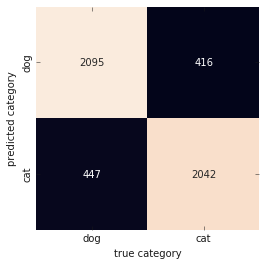
\includegraphics[width=0.8\linewidth]{img/autokeras-5-confusion.png}
        \caption{Confusion matrix.}
        \label{fig:confusion-autokeras-5}
    \end{subfigure}
    \begin{subfigure}{0.5\textwidth}
        \centering
        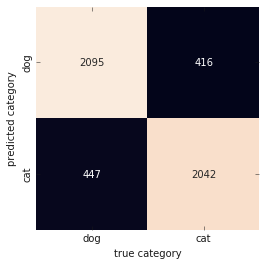
\includegraphics[width=0.8\linewidth]{img/autokeras-5-confusion.png}
        \caption{Confusion matrix.}
        \label{fig:confusion-autokeras-10}
    \end{subfigure}
    \begin{subfigure}{0.5\textwidth}
        \centering
        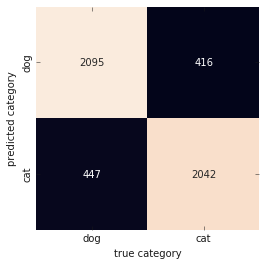
\includegraphics[width=0.8\linewidth]{img/autokeras-5-confusion.png}
        \caption{Confusion matrix.}
        \label{fig:confusion-autokeras-50}
    \end{subfigure}
    \caption{Confusion matrices voor de verschillende modellen.}
    \label{fig:confusion-matrices-autokeras}
\end{figure}

\begin{figure}
    \centering
    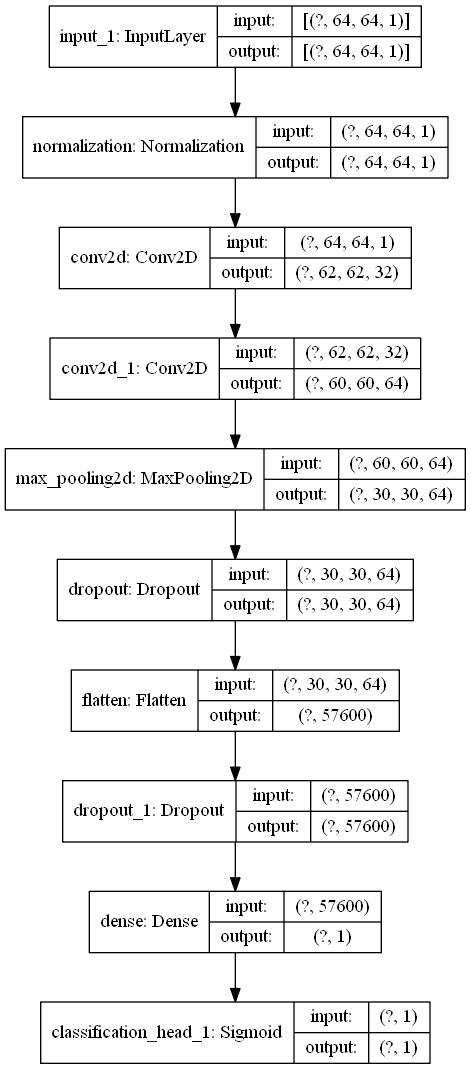
\includegraphics[width=0.7\linewidth]{img/model-samenvatting.png}
    \caption{Mogelijke lagenstructuur van een model.}
    \label{fig:layer-autokeras}
\end{figure}

\begin{figure}
    \centering
    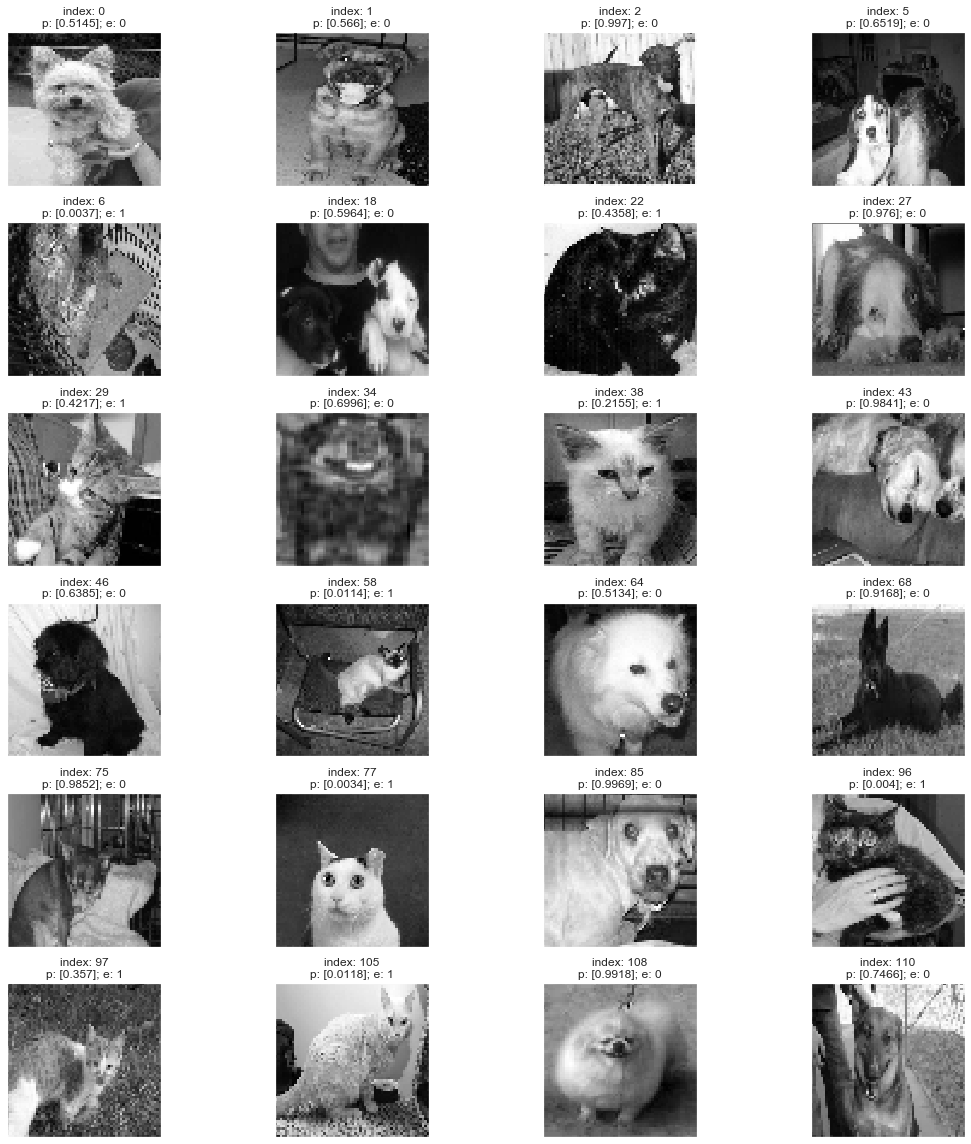
\includegraphics[width=0.7\linewidth]{img/autokeras-5-wrong-images.png}
    \caption{Verkeerd voorspelde afbeeldingen.}
    \label{fig:wrong-prediction-autokeras}
\end{figure}

\section{Requirements}